\chapter{Experiment setup}
\lhead{Experiment setup}
\rhead{Radu-George Rusu}
\label{ExperimentSetup}

This chapter will present the thought process and the setup that was used to run the experiments on the dataset presented in Chapter \ref{DatasetChapter}.

\section{Initial idea}

Taking a high level look through the training data set, a general case can be seen: pictures are taken at sea (no port in site) and as such, they are also conceived from water and ships (which can divide pixels in two group as shown in image \ref{ShipExampleAtSea}). If the images are moved into grayscale, and their histogram is computed (\ref{ImageHistogram}), then the pixels of the image can be split into two groups, both generated by a Gaussian distribution, which will also give the ship/no-ship classification. This problem is a classical problem that can be solved using EM algorithm.

\begin{figure}[h]
	\centering
	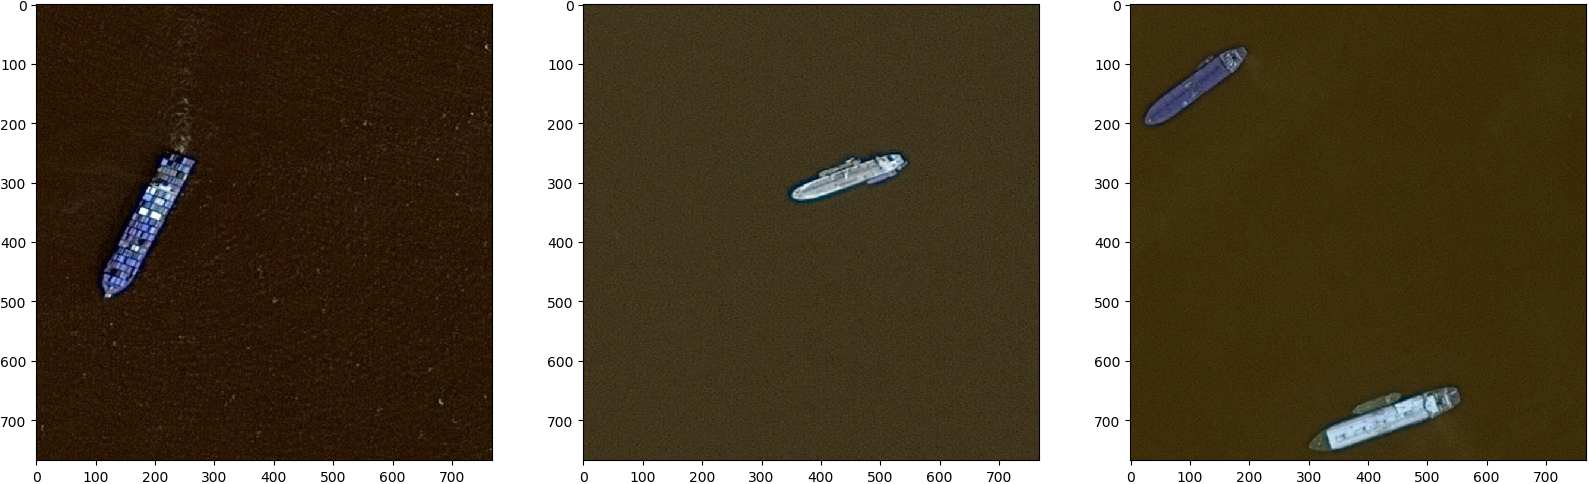
\includegraphics[height=0.2\textheight]{Pictures/002ShipExampleatSea.png}
	\caption{Ships at sea}
	\label{ShipExampleAtSea}
\end{figure}

\begin{figure}[h]
	\centering
	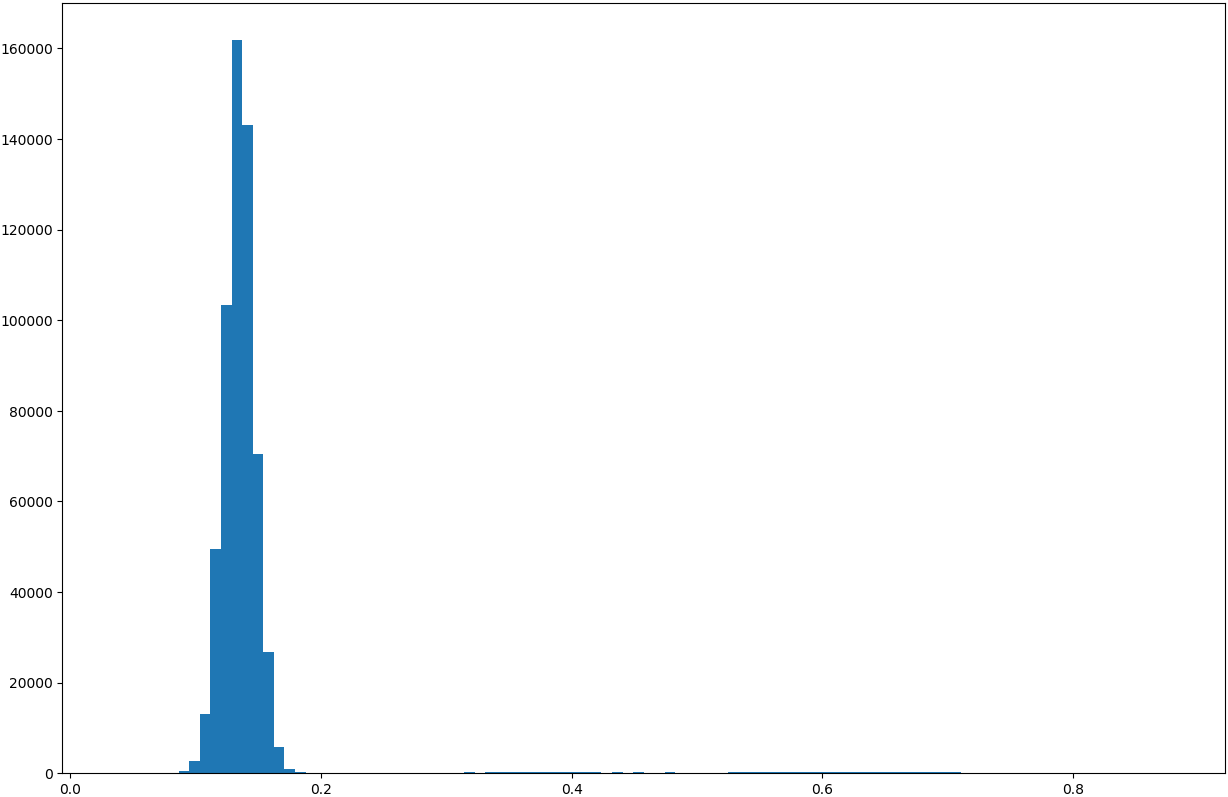
\includegraphics[width=\textwidth]{Pictures/005ImageHistogram.png}
	\caption{Histogram of grayscale at sea image}
	\label{ImageHistogram}
\end{figure}

\section{Expectation-Maximization}
For the rest of this section the following notations will be used:
\begin{table}[H]
	\centering
	\begin{tabular}{cp{0.8\textwidth}}
		$\mathbf{p(x_i)}$ & probability of the pixel $i$ \\ 
		$\mathbf{\mathcal{N} (x_i | \mu_s , \sigma_s)}$ & PDF value of pixel $i$ generated by the ship Gaussian distribution \\
		$\mathbf{\mathcal{N} (x_i | \mu_b , \sigma_b)}$ & PDF value of pixel $i$ generated by the background Gaussian distribution \\
		$\mathbf{G_s}$ & random variable that represents the presence of ships in the image\\
		$\mathbf{G_b}$ & random variable that represents the presence of background in the image\\
		$\mathbf{n}$ & number of pixels in the image 
	\end{tabular}
	\caption{Notations}\label{notations}
\end{table}
In order to apply EM to our problem, some adaptations must be done. First, we will be considering two random variables $G_s$ and $G_b$, both in $[0, 1]$, which will represent the presence of ship, respectively background in the image. The hidden variables in this problem will be some random variables that assign every pixel either to the ship group or background group. Also, considering the observation from the beginning of this section, the value of every pixel will be a probability generated by the two Gaussians as follows:
$$ p(x_i) = \mathcal{N}(x_i | \mu_s, \sigma_s) P(G_s) + \mathcal{N}(x_i | \mu_b, \sigma_b) P(G_b) $$

\subsection{E-Step}

The likelihood of the data will be computed as follows:

$$L = \prod_{i=1}^{n} p(x_i) = \prod_{i=1}^{n} \mathcal{N}(x_i | \mu_s, \sigma_s) P(G_s) + \mathcal{N}(x_i | \mu_b, \sigma_b) P(G_b)$$

Next we compute the mean of the likelihood for this iteration:
$$Q(h | h^{(t)}) = E_{P(G | x, h^{(t)})}\bigg[\prod_{i=1}^{n} \mathcal{N}(x_i | \mu_s, \sigma_s) P(G_s) + \mathcal{N}(x_i | \mu_b, \sigma_b) P(G_b)\bigg]$$
$$=\prod_{i=1}^{n} E_{P(G | x, h^{(t)})}\bigg[\mathcal{N}(x_i | \mu_s, \sigma_s) P(G_s) + \mathcal{N}(x_i | \mu_b, \sigma_b) P(G_b)\bigg] $$
$$=\prod_{i=1}^{n}E_{P(G | x, h^{(t)})}\bigg[\mathcal{N}(x_i | \mu_s, \sigma_s) P(G_s)\bigg] + E_{P(G | x, h^{(t)})}\bigg[\mathcal{N}(x_i | \mu_b, \sigma_b) P(G_b)\bigg] $$
$$=\prod_{i=1}^{n} \mathcal{N}(x_i | \mu_s, \sigma_s) E_{P(G | x, h^{(t)})} P(G_s) + \mathcal{N}(x_i | \mu_b, \sigma_b) E_{P(G | x, h^{(t)})} P(G_b) $$

Now the estimation for the $P(G_s)$ and $P(G_b)$ must be computed considering that:
$$P(G_s) = \frac{1}{n} \sum_{t = 1}^{n}P(G_s | x_i)$$
$$P(G_b) = \frac{1}{n} \sum_{t = 1}^{n}P(G_b | x_i)$$
which leads to:
$$E_{P(G | x, h^{(t)})} P(G_s) = \sum_{i=1}^{n} E_{P(G | x, h^{(t)})} P(G_s | x_i) $$
$$E_{P(G | x, h^{(t)})} P(G_b) = \sum_{i=1}^{n} E_{P(G | x, h^{(t)})} P(G_b | x_i) $$

The ML estimation of the above elements is as follows \cite{EMObjectConcealement}:
$$E_{P(G | x, h^{(t)})} P(G_s | x_i) = \frac{\mathcal{N}(x_i | \mu_s^{(t)}, \sigma_s^{(t)}) P(G_s)^{(t)}}{\mathcal{N}(x_i | \mu_s^{(t)}, \sigma_s^{(t)}) P(G_s)^{(t)} + \mathcal{N}(x_i | \mu_b^{(t)}, \sigma_b^{(t)}) P(G_b)^{(t)}}	$$

$$E_{P(G | x, h^{(t)})} P(G_b | x_i) = \frac{\mathcal{N}(x_i | \mu_b^{(t)}, \sigma_b^{(t)}) P(G_b)^{(t)}}{\mathcal{N}(x_i | \mu_s^{(t)}, \sigma_s^{(t)}) P(G_s)^{(t)} + \mathcal{N}(x_i | \mu_b^{(t)}, \sigma_b^{(t)}) P(G_b)^{(t)}}	$$

\subsection{M-Step}
At this point, considering the previous section, we have a form for the expectation of the likelihood function, so the Maximization step can be applied. By taken the above formulas and computing the derivatives based on the parameters we obtain the following actualization rules \cite{EMObjectConcealement}: \\

\begin{table}[H]
	\centering
	\begin{tabular}{cc}
		\begin{minipage}{0.5\textwidth}
			$$\mu_s^{(t+1)} = \frac{\sum_{i=1}^{n}P(G_s | x_i) * x_i}{\sum_{i=1}^{n}  P(G_s | x_i)}$$
		\end{minipage} &
		\begin{minipage}{0.5\textwidth}
			$$\mu_b^{(t+1)} = \frac{\sum_{i=1}^{n}P(G_b | x_i) * x_i}{\sum_{i=1}^{n} P(G_b | x_i)}$$ 
		\end{minipage} \\ 
		\\
		\begin{minipage}{0.5\textwidth}
			$$\sigma_s^{(t+1)} = \frac{\sum_{i=1}^{n} P(G_s | x_i) (x_i - \mu_s^{(t)})^2}{\sum_{i=1}^{n} P(G_s | x_i)}$$
		\end{minipage} &
		\begin{minipage}{0.5\textwidth}
			$$\sigma_b^{(t+1)} = \frac{\sum_{i=1}^{n} P(G_b | x_i) (x_i - \mu_b^{(t)})^2}{\sum_{i=1}^{n} P(G_b | x_i)}$$
		\end{minipage} \\
		\\
		\begin{minipage}{0.5\textwidth}
			$$P(G_s)^{(t+1)} = \frac{1}{n} \sum_{t = 1}^{n}P(G_s | x_i)$$
		\end{minipage} &
		\begin{minipage}{0.5\textwidth}
			$$P(G_b)^{(t+1)} = \frac{1}{n} \sum_{t = 1}^{n}P(G_b | x_i)$$
		\end{minipage} \\
	\end{tabular}
\end{table}

The initialization values for the EM parameters were given as random between $0$ and $1$, for $\mu$ and $\sigma$. The $P(G_b)$ had an initial value of $0.9$ and $P(G_s)$ a value of $0.1$, since we expect to have more background than ships in an image. In order to stop the algorithm, a maximum iteration value of 12 was used, without any other restrictions. Parameter learning was executed on a resized ($256\times256$) for performance reasons, and the classification phase was run on the full-size image. After the parameters were computed, the following rule was used to classify pixels as either ship or background:
\begin{itemize}
	\item if $P(G_s | x_t) \geq P(G_b | x_t)$ then classify $x_t$ as \textbf{ship}
	\item if $P(G_s | x_t) < P(G_b | x_t)$ then classify $x_t$ as \textbf{background}
\end{itemize}
Before applying the EM algorithm, all images were converted to grayscale so that every pixel has only one characteristic value and not 3, like in the RGB format. Another preprocessing technique used was a Gaussian filter with the purpose of smoothing the edges in the picture. 


\subsection{EM results}
\label{emres}
After applying the EM algorithm over a subset of images we obtain results as shown in \ref{init_result}.

\begin{figure}[h]
	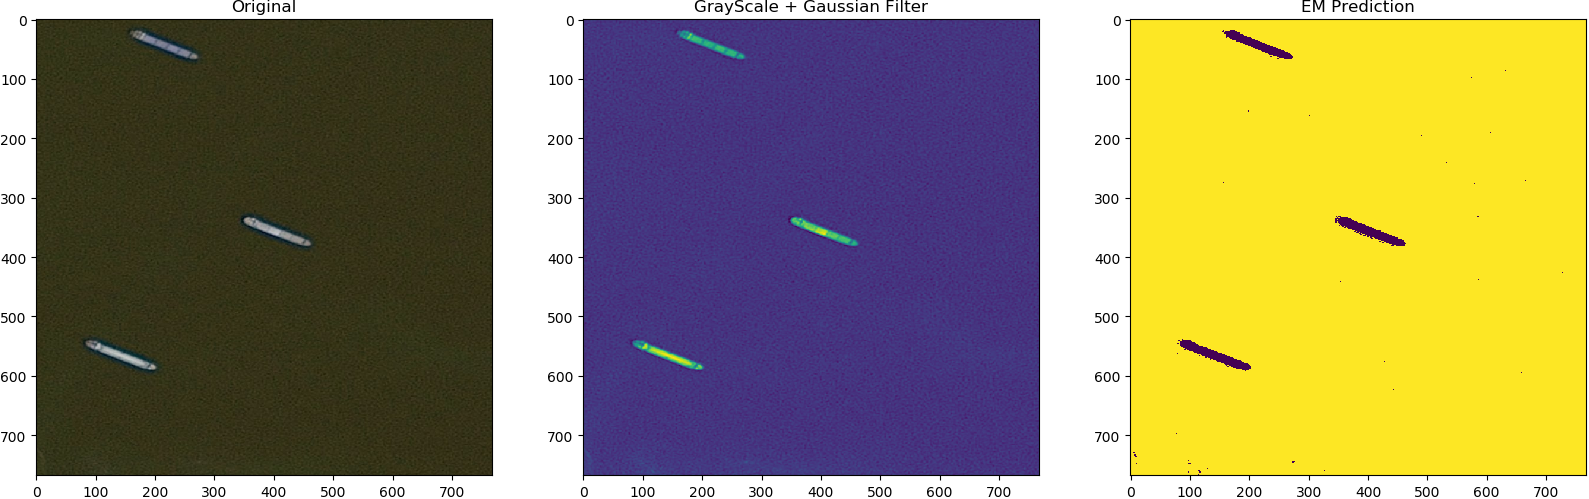
\includegraphics[width=\textwidth]{Pictures/009Ex1.png}\\
	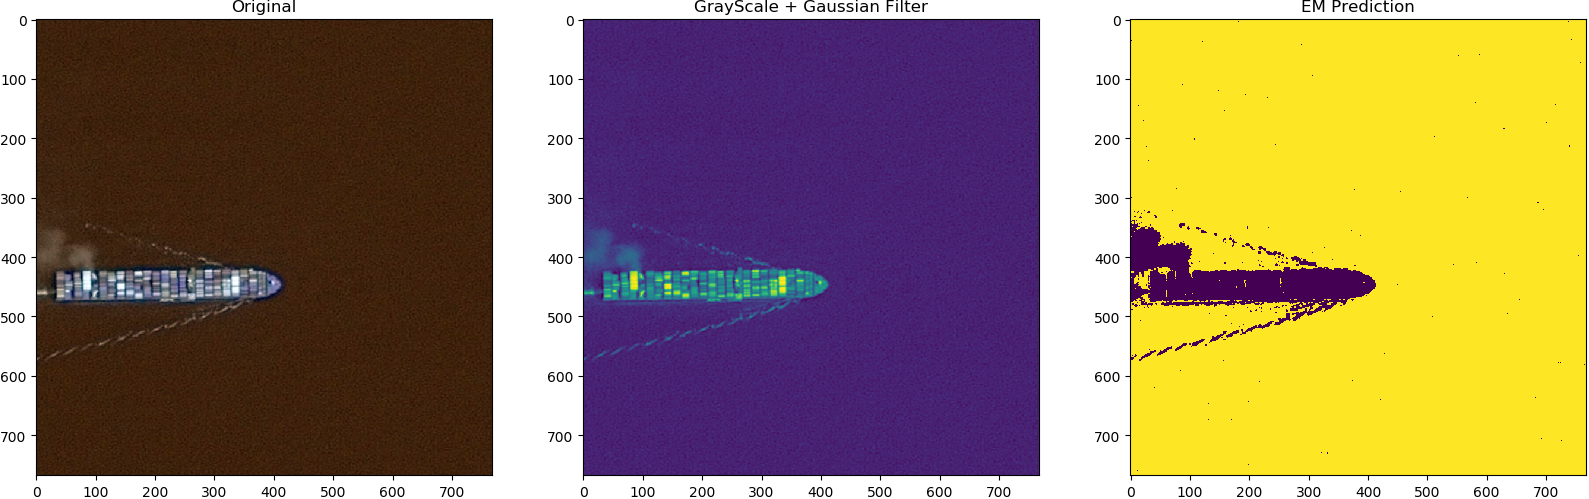
\includegraphics[width=\textwidth]{Pictures/009Ex2.png}\\
	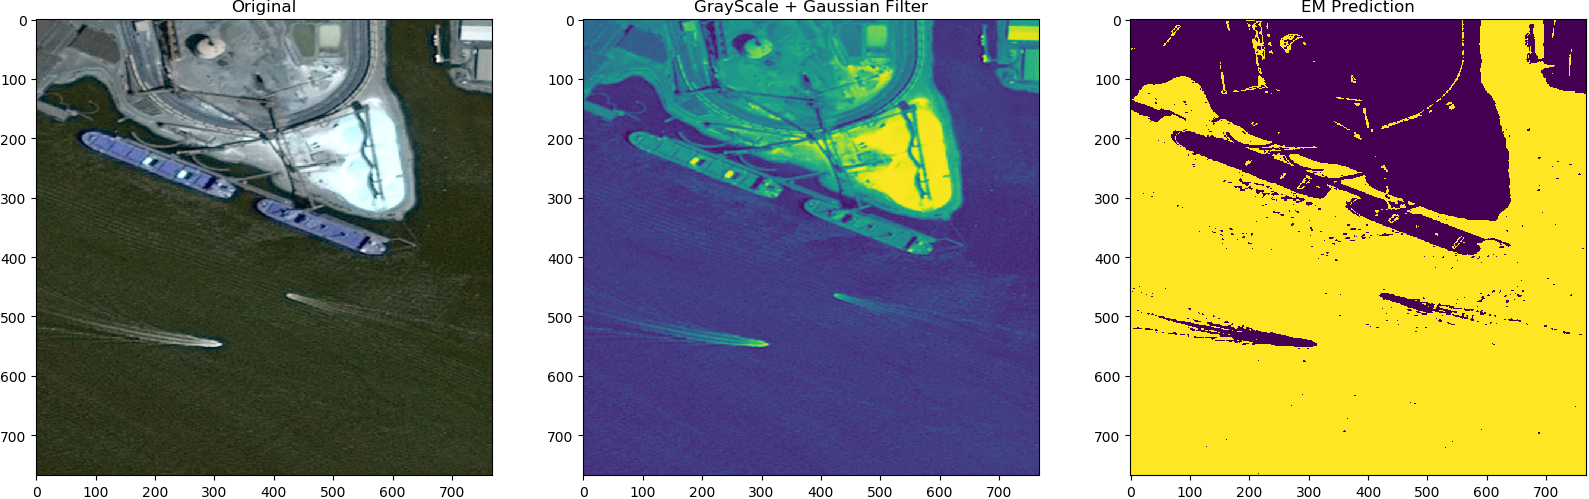
\includegraphics[width=\textwidth]{Pictures/009Ex3.png}
	\caption{Initial Results}
	\label{init_result}
\end{figure}

It can be observed that in "at sea" pictures, the algorithm behaves quite good
(although it still predicts some pockets of pixels that are not ships), but in
the port pictures the algorithm detects the port as being a ship as well.
Also, because the algorithm enforce that every pixel is generated by the
formula specified earlier, in case of no-ship picture this algorithm will still
detect ships.

After this steps, 3 main caveats of the EM algorithm have been identified:
\begin{itemize}
	\item [1.] the algorithm is classifying pixels in images that have no ship (the algorithm is not able to distinguish this particular case) \textbf{(P1)}
	\item [2.] the algorithm is classifying small pockets of pixels as ship (usually waves that visually distinguish themselves from the rest of the water) \textbf{(P2)}
	\item [3.] in the images that have ports, the algorithm identifies the port pixels as being ships (mainly because of the color similarity between them) \textbf{(P3)}
\end{itemize}

\section{Region Proposal Solution}
\label{regPropSol}
Since the EM algorithm by itself had the caveats mentioned in \ref{emres}, a pipeline \ref{arch1} around the algorithm was developed.
To solve \textbf{(P1)} a Residual Network (with a ResNet34 architecture \cite{ResNetPaper}) was used for classifying the images, in images with ships and with no ships. Using this, the EM algorithm could be ran, only on the images that are certain to have ships. The network was train on \textbf{10000} images, plus rotation with -90 and 90 degrees, randomly selected from the train set of the initial problem.

\begin{figure}[h]
	\centering
	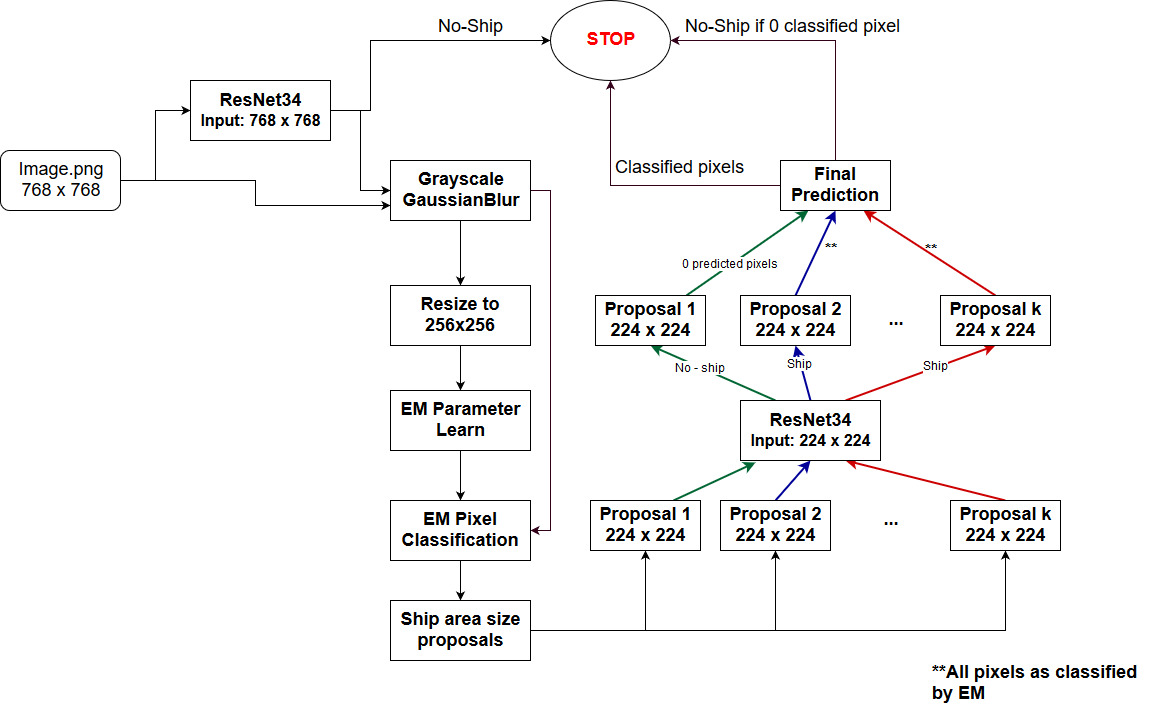
\includegraphics[angle=90,height=0.8\textheight]{Pictures/010Architecture1.jpg}
	\caption{Region Proposal}
	\label{arch1}
\end{figure}

After this phase, on the images classified as ship images, the EM algorithm was ran. In order to solve \textbf{(P2)}, a de-noising technique was applied on the image result. The fast de-noising Nl means from cv2 library was chosen, which helps removing small pockets of isolated pixels, and also smoothen the edges of the ships. The method is applied for each pixel, by taken a surrounding area of the target pixel and averaging it with similar areas in the image.

Finally, in the third phase, another Residual Network was used in order to remove the ship labels from port pixels. This is a more difficult issue to solve, since ports have a color scheme really similar to ships.
\begin{itemize}
	\item First we split the EM predicted image in 25 crops, of size $224 \times 224$.
	\item Only the windows that have at least 35 (\ref{shipzisepixeltable}) pixels predicted as ship will be considered as a possible valid prediction.
	\item This Residual Network also used the ResNet34 architecture \cite{ResNetPaper}, and was trained on $224\times224$ random crops ($\sim \mathbf{50000}$, taken the same way as the selection for prediction), that is capable of classifying the idea of ship/no-ship.
\end{itemize}

\section{Region Proposal Example Run}
The following figures shows a picture in different stages of processing:
\begin{enumerate}
	\item \ref{orig_pic} - the input image of the algorithm (left), the image after the Gaussian filter was apply and the encoding was moved to grayscale (right)
	\item \ref{em_pic} - the classification result after the em algorithm where the yellow pixels are background, and the purple one are ships(left), and the em result after the de-noising technique has been applied(right)
	\item \ref{propose_pic} - the 9 propose regions for second classification
	\item \ref{final_result_pic} - the final result compared to the initial picture
\end{enumerate}

\begin{figure}[h]
	\centering
	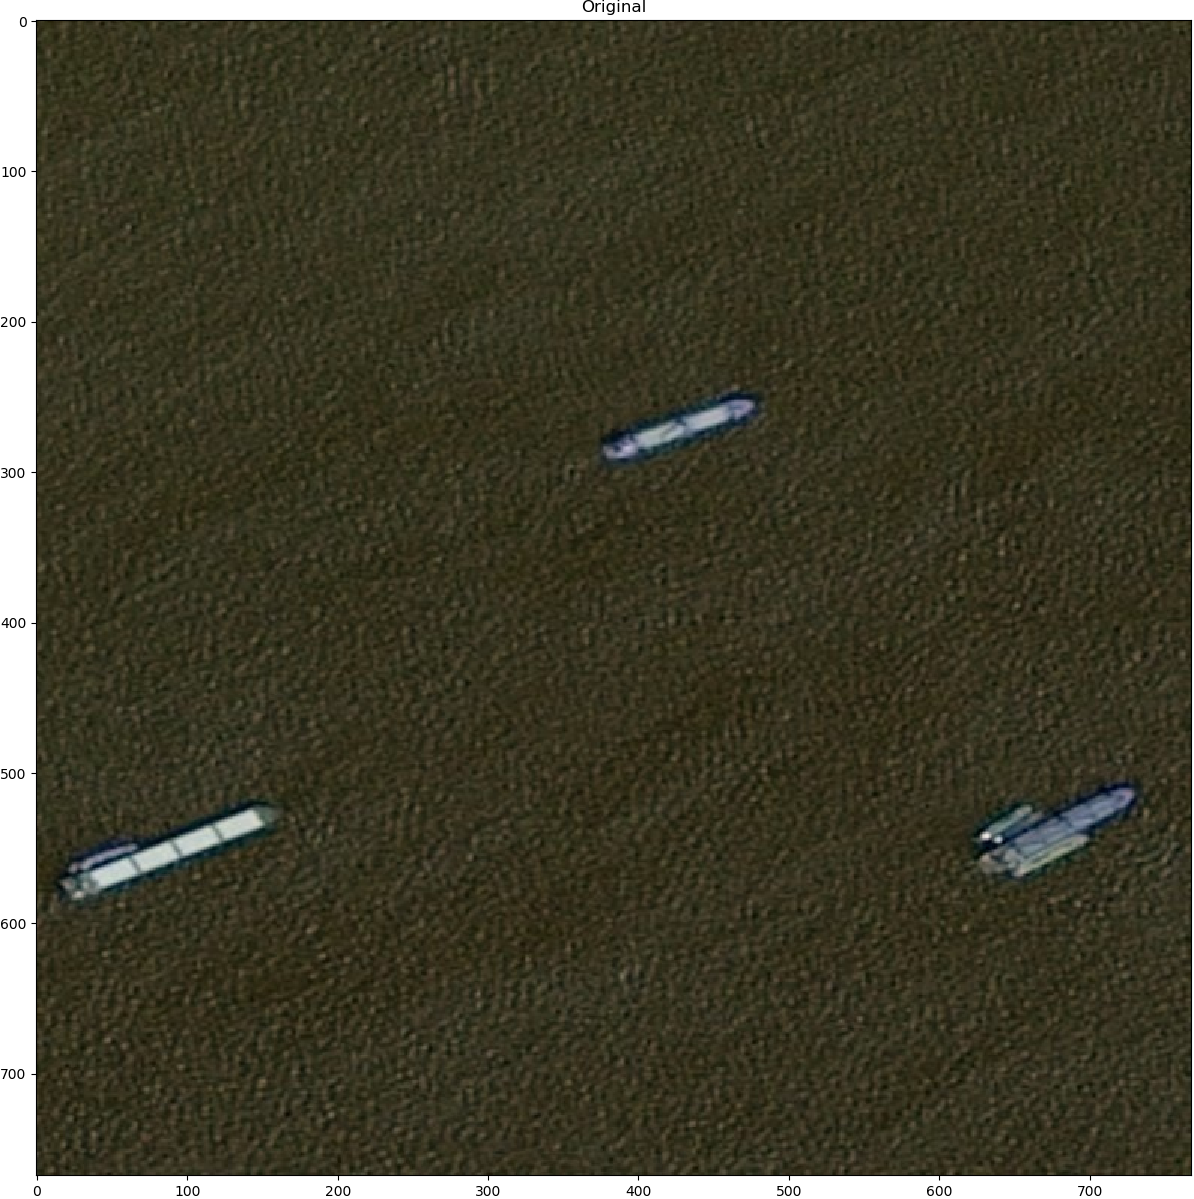
\includegraphics[width=0.45\textwidth]{Pictures/011Original.png}
	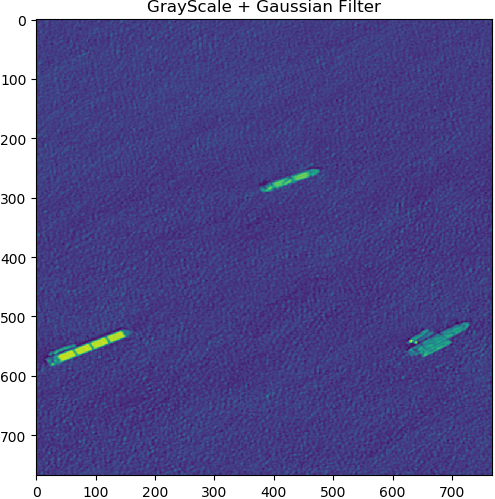
\includegraphics[width=0.45\textwidth]{Pictures/011GrayScale.png}
	\caption{Input/Original Picture, Grayscale and Gaussian Filtering}
	\label{orig_pic}
\end{figure}

\begin{figure}[h] 
	\centering
	\includegraphics[width=0.45\textwidth]{Pictures/011EMPred.png}
	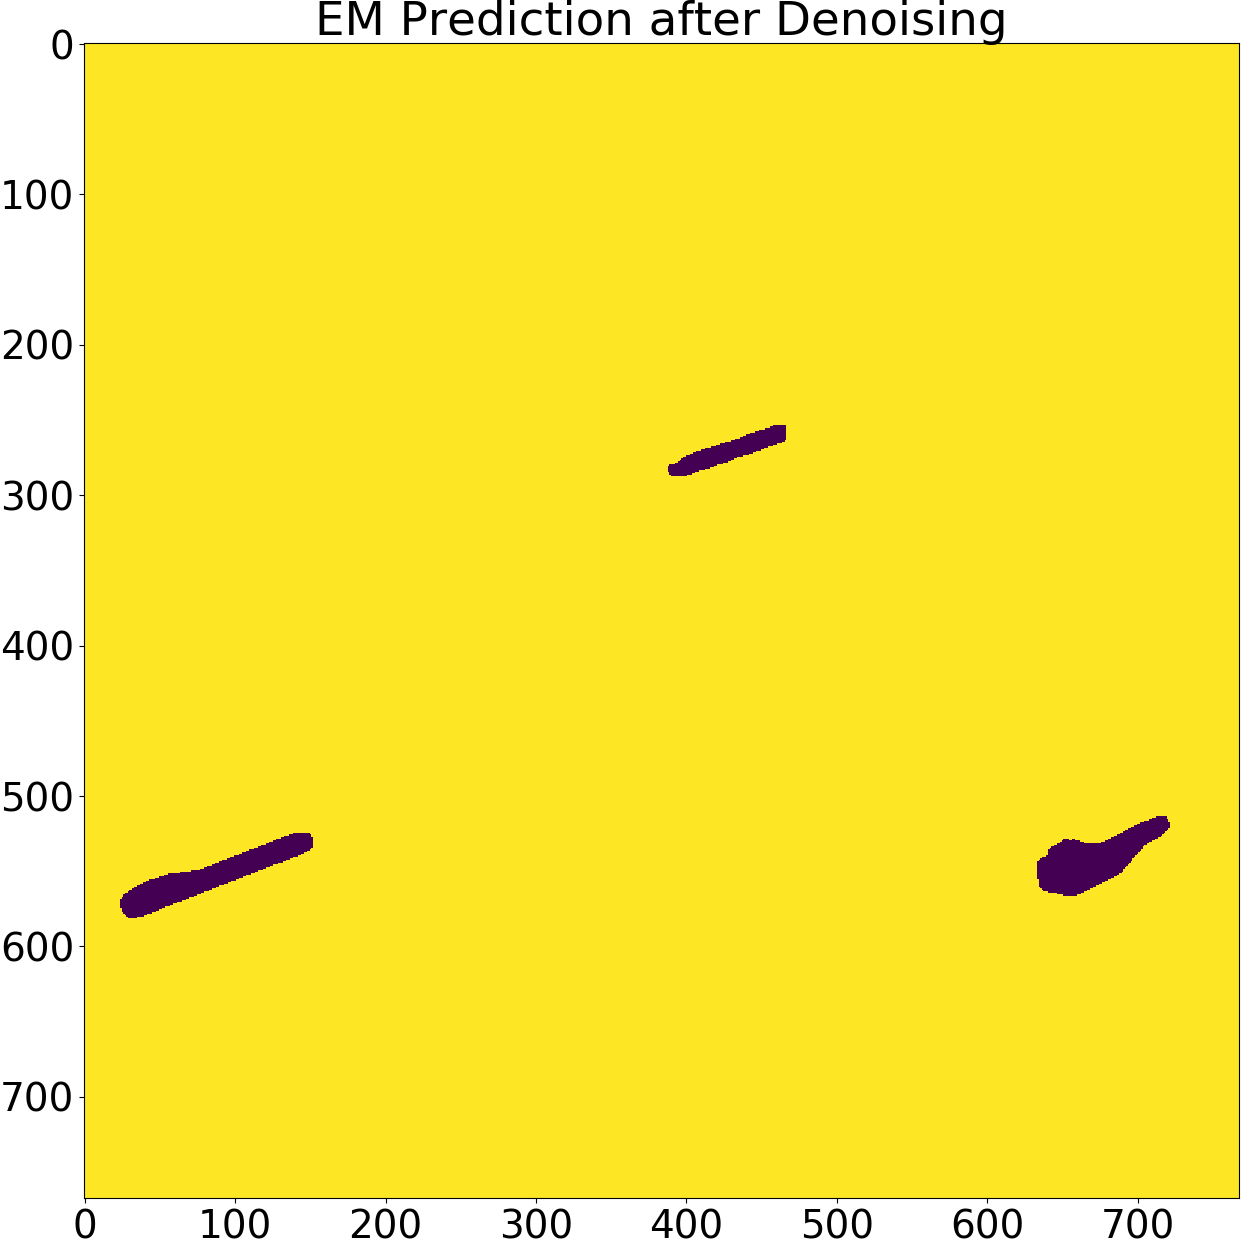
\includegraphics[width=0.45\textwidth]{Pictures/011Denoising.png}
	\caption{EM Result before and after denoising}
	\label{em_pic}
\end{figure}
\begin{figure}[h]
	\centering
	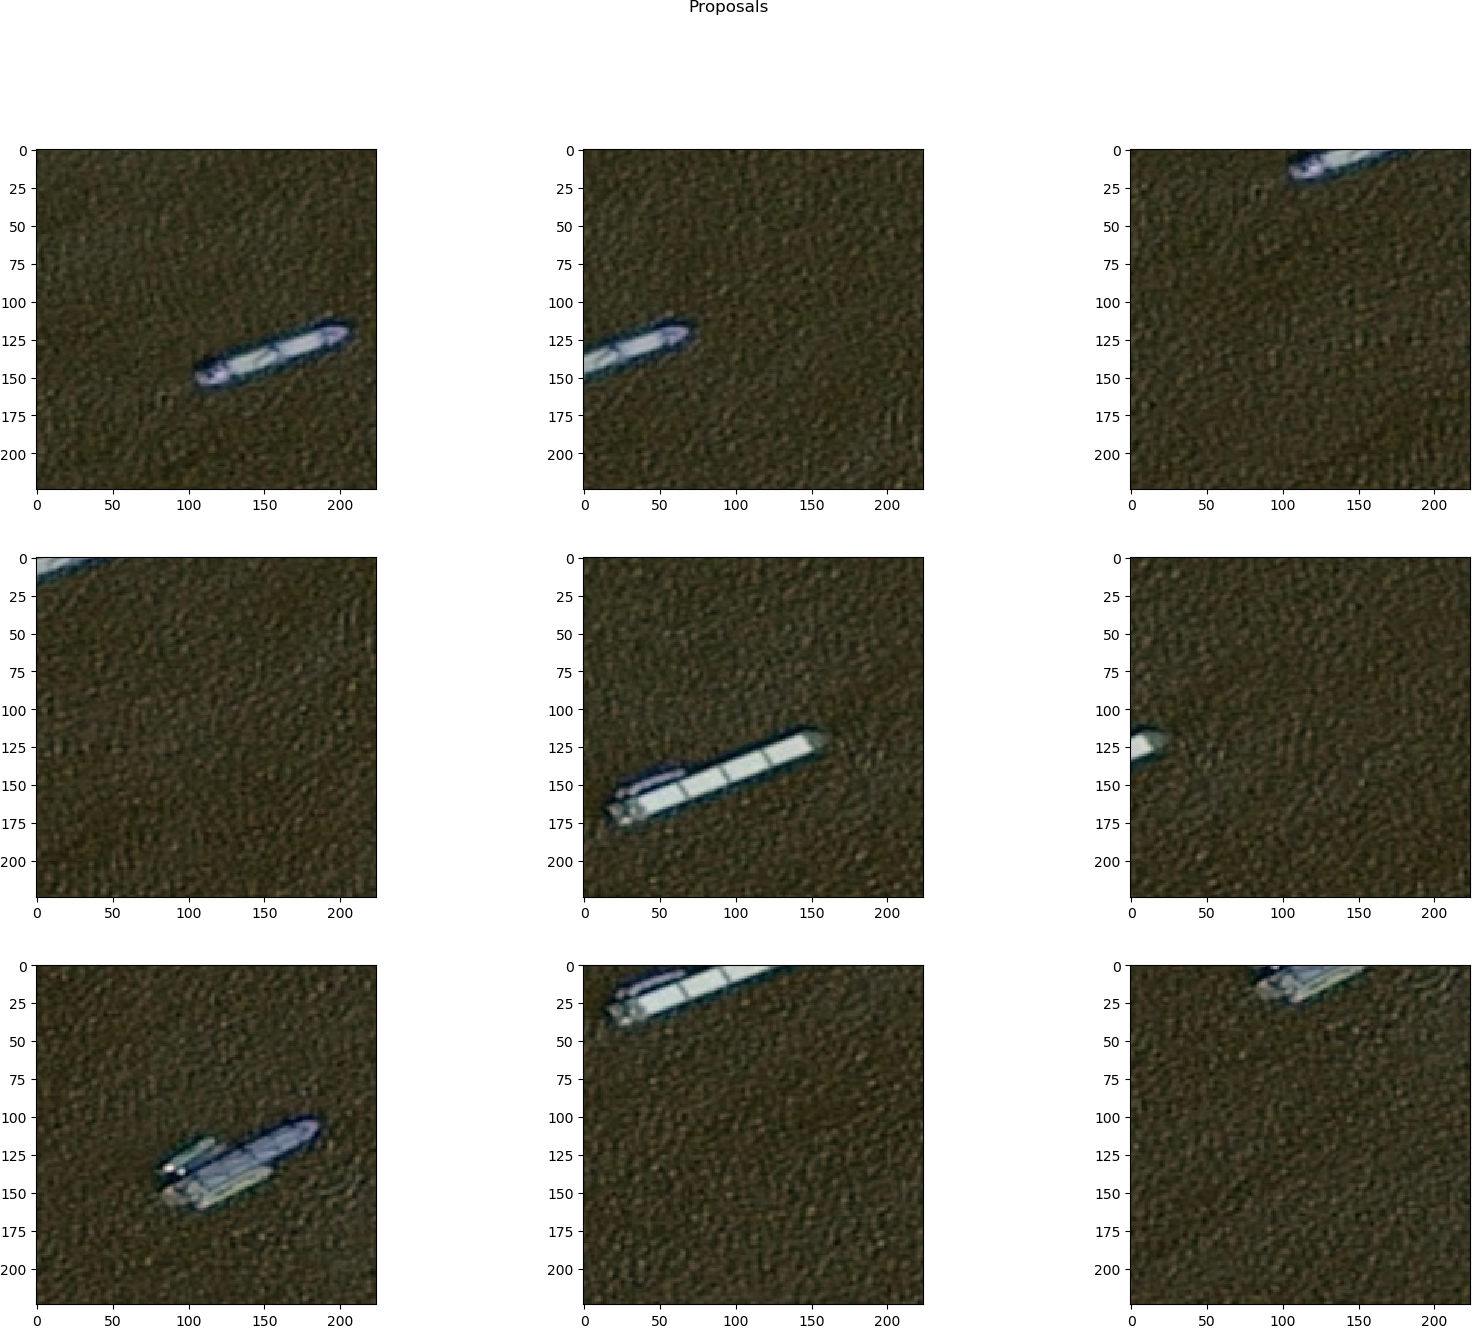
\includegraphics[height=0.6\textheight]{Pictures/011Proposals.png}\\
	\caption{9/25 proposed regions}
	\label{propose_pic}
\end{figure}
\begin{figure}[H]
	\centering
	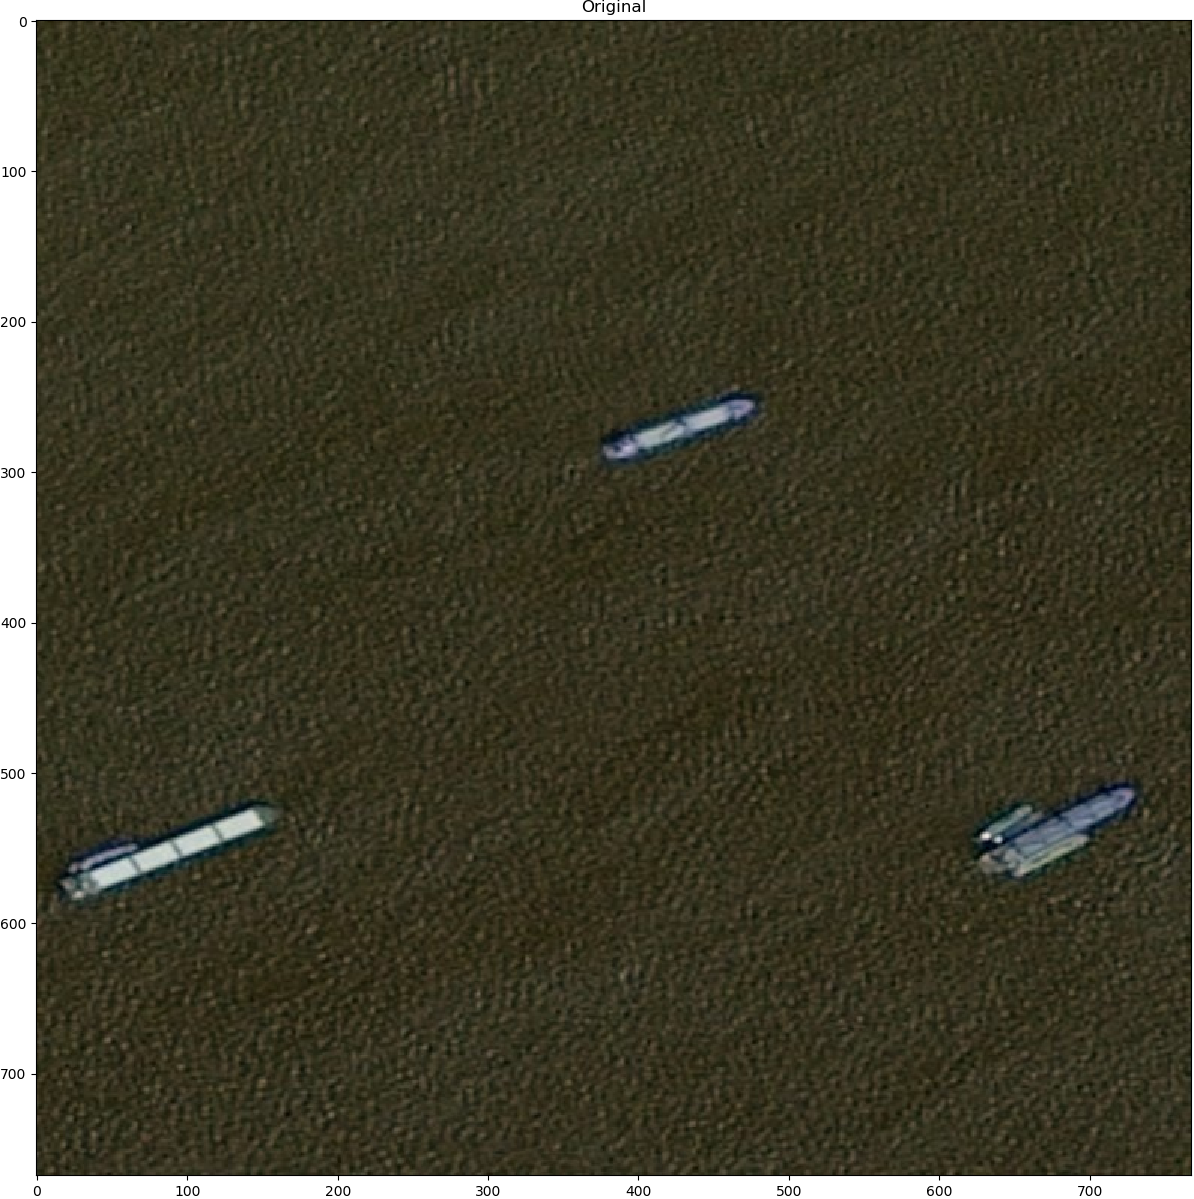
\includegraphics[width=0.45\textwidth]{Pictures/011Original.png}
	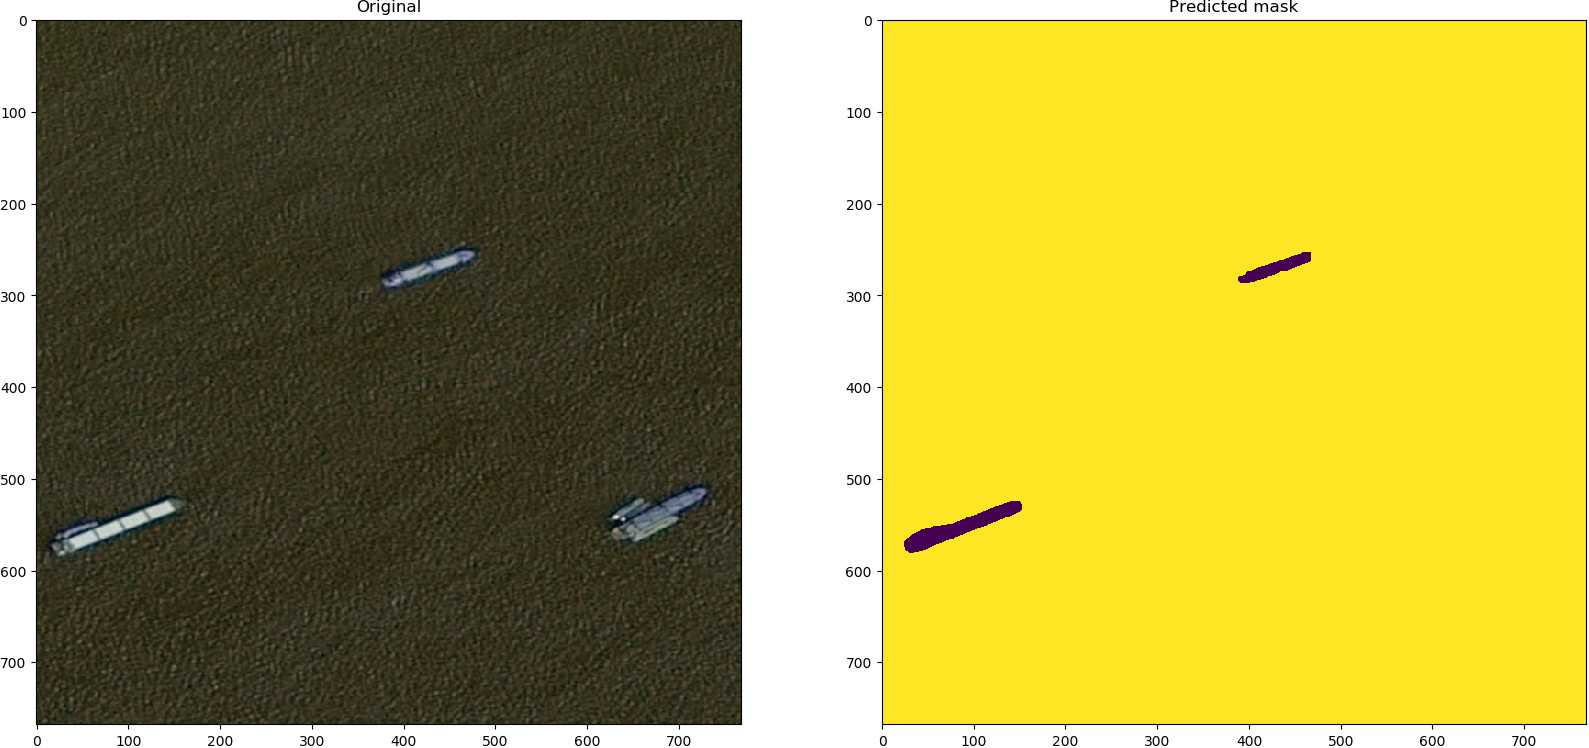
\includegraphics[width=0.45\textwidth]{Pictures/011FinalResult.png}
	\caption{Final Result}
	\label{final_result_pic}
\end{figure}


\section{U-Net Solution}
Another solution for solving the \textbf{(P3)}, was the usage of U-Nets \cite{Unet}. As show in \ref{UnetArch} the initial part of the classification stays the same as in the Region Proposal Solution. This solutions changes after the EM classification is finished. Instead of extracting proposed region for another classification, the pixels that were classified as background are turned black (Pixel Exclusion phase) in the original image, and afterwards the image is sent through a U-Net and a Gaussian smoothing for the final prediction.
\begin{figure}[h]
	\centering
	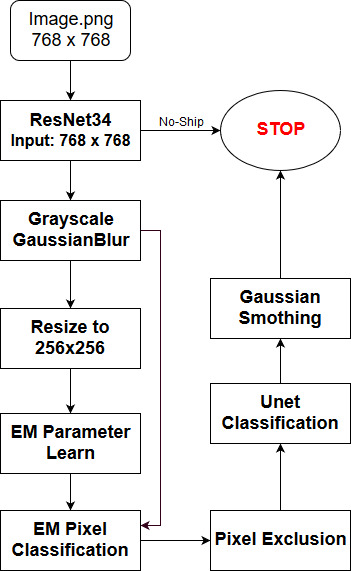
\includegraphics[width=0.5\textwidth]{Pictures/013UnetArchitecture.jpg}\\
	\caption{U-Net}
	\label{UnetArch}
\end{figure}

For the training of the U-net, a modified version of the $F_2$ score was used. Since inside a model training, the loss function must be minimized, and in the case of the $F_2$ score, a higher score means a better prediction, a loss function equal to $-F_2$ was used. The model was trained until the loss function reached the value of $-0.2$. On every training phase, the model pass thorough 10 epochs, and for each epoch 9 training steps were executed on the model. For every epoch 48 images were randomly selected from the training set.

\section{U-Net Example Run}
The following figures shows a picture in different stages of processing:
\begin{enumerate}
	\item \ref{orig_pic_unet} - as in the Region Proposal Solution the initial steps doesn't change. The picture is moved to grayscale, and the Gaussian filter is applied.
	\item \ref{em_pic_unet} - the classification result after the em algorithm where the yellow pixels are background, and the purple one are ships (left), and new image with the pixels classified as background are colored as black in the original image (right).
	\item \ref{final_result_pic_unet} - the final result compared to the initial picture. The final result is obtained by inserting the exclusion pixel image in the U-Net network.
\end{enumerate}
\begin{figure}[h]
	\centering
	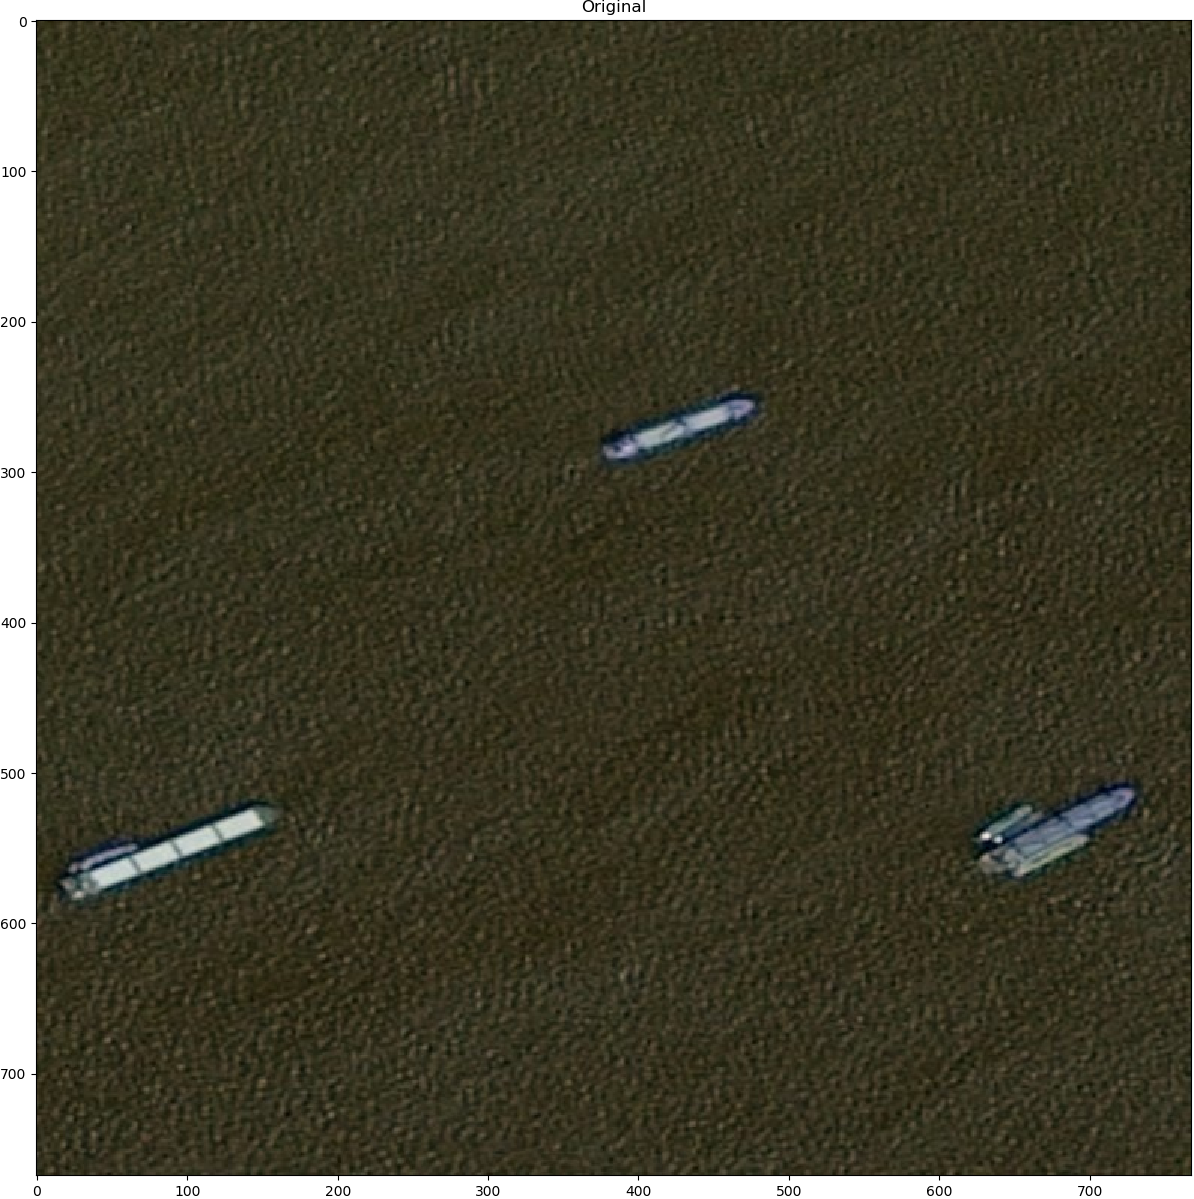
\includegraphics[width=0.45\textwidth]{Pictures/011Original.png}
	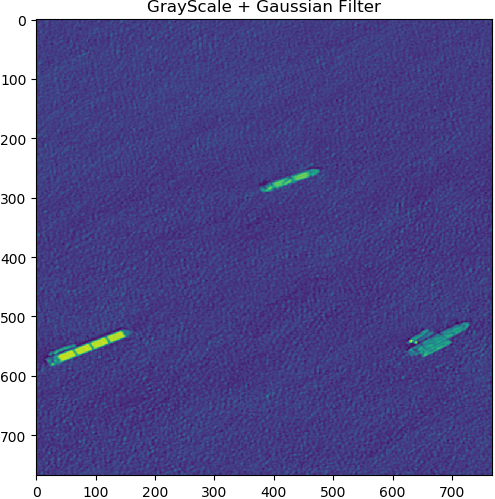
\includegraphics[width=0.45\textwidth]{Pictures/011GrayScale.png}
	\caption{Input/Original Picture, Grayscale and Gaussian Filtering}
	\label{orig_pic_unet}
\end{figure}
\begin{figure}[h] 
	\centering
	\includegraphics[width=0.45\textwidth]{Pictures/011EMPred.png}
	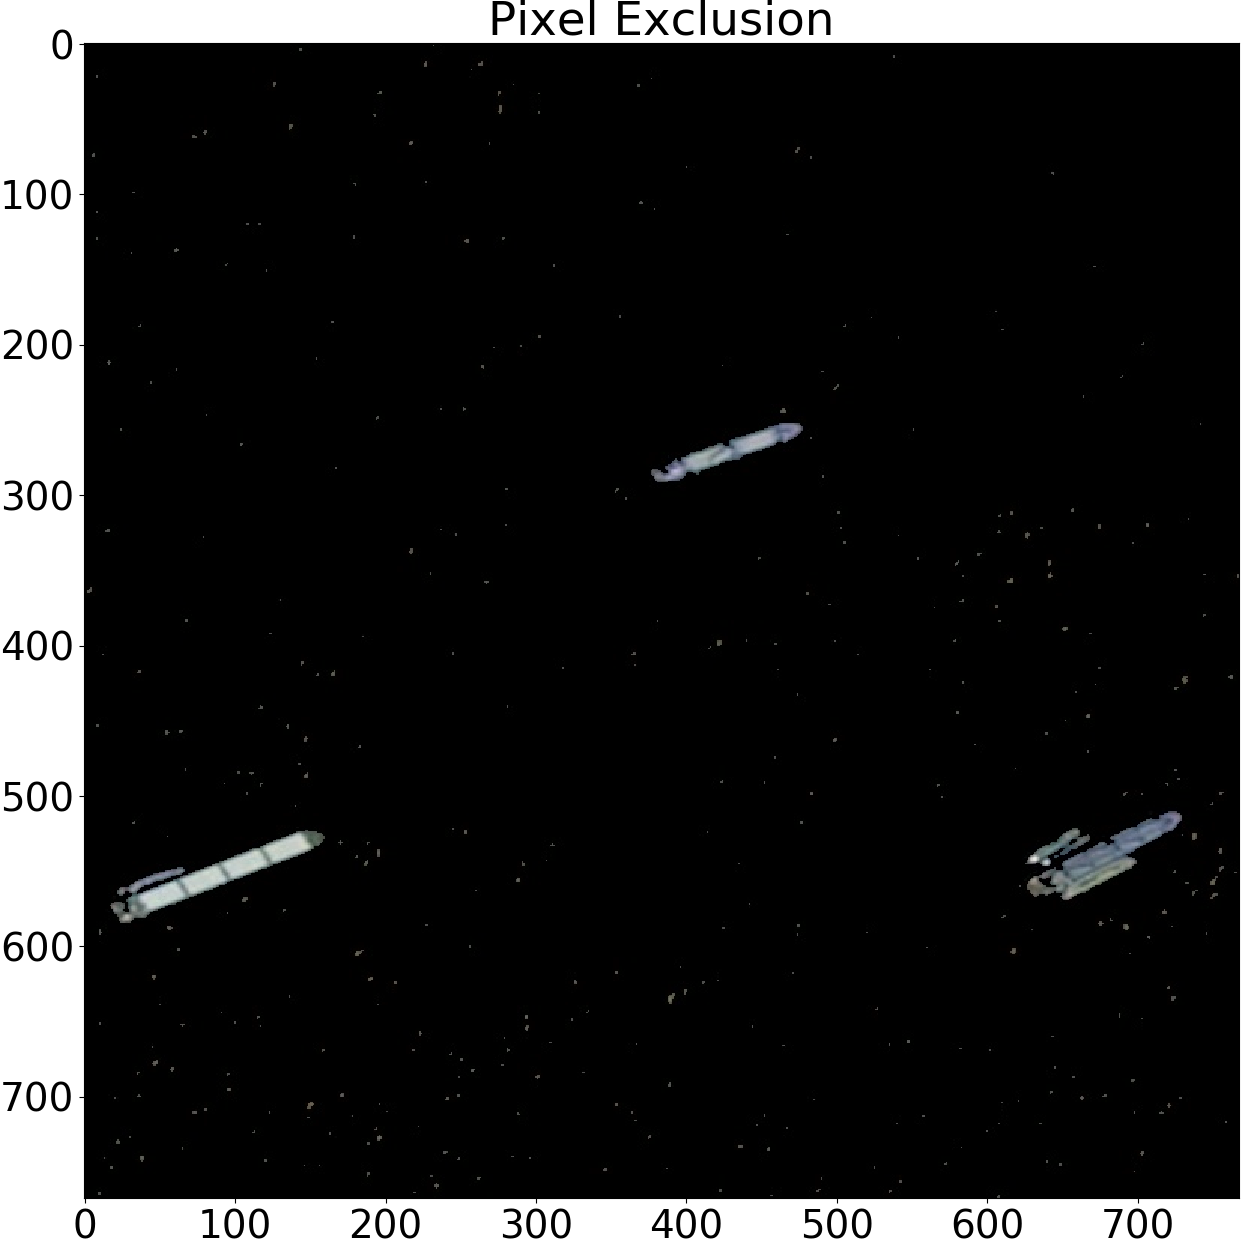
\includegraphics[width=0.45\textwidth]{Pictures/014PixelExclusion.png}
	\caption{EM Result and Pixel Exclusion}
	\label{em_pic_unet}
\end{figure}
\begin{figure}[H]
	\centering
	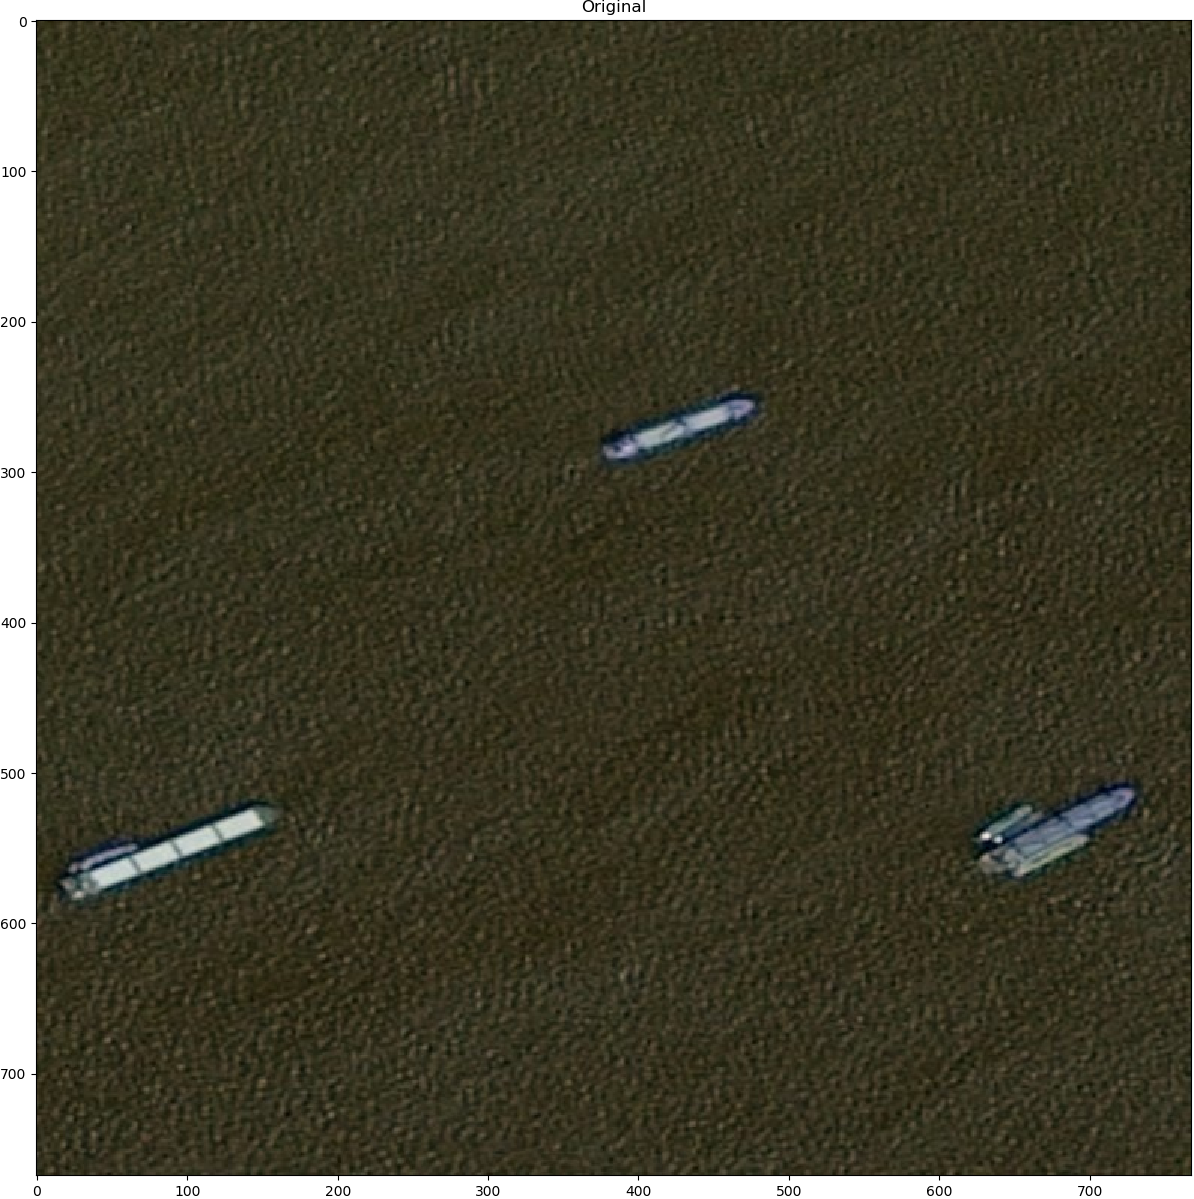
\includegraphics[width=0.45\textwidth]{Pictures/011Original.png}
	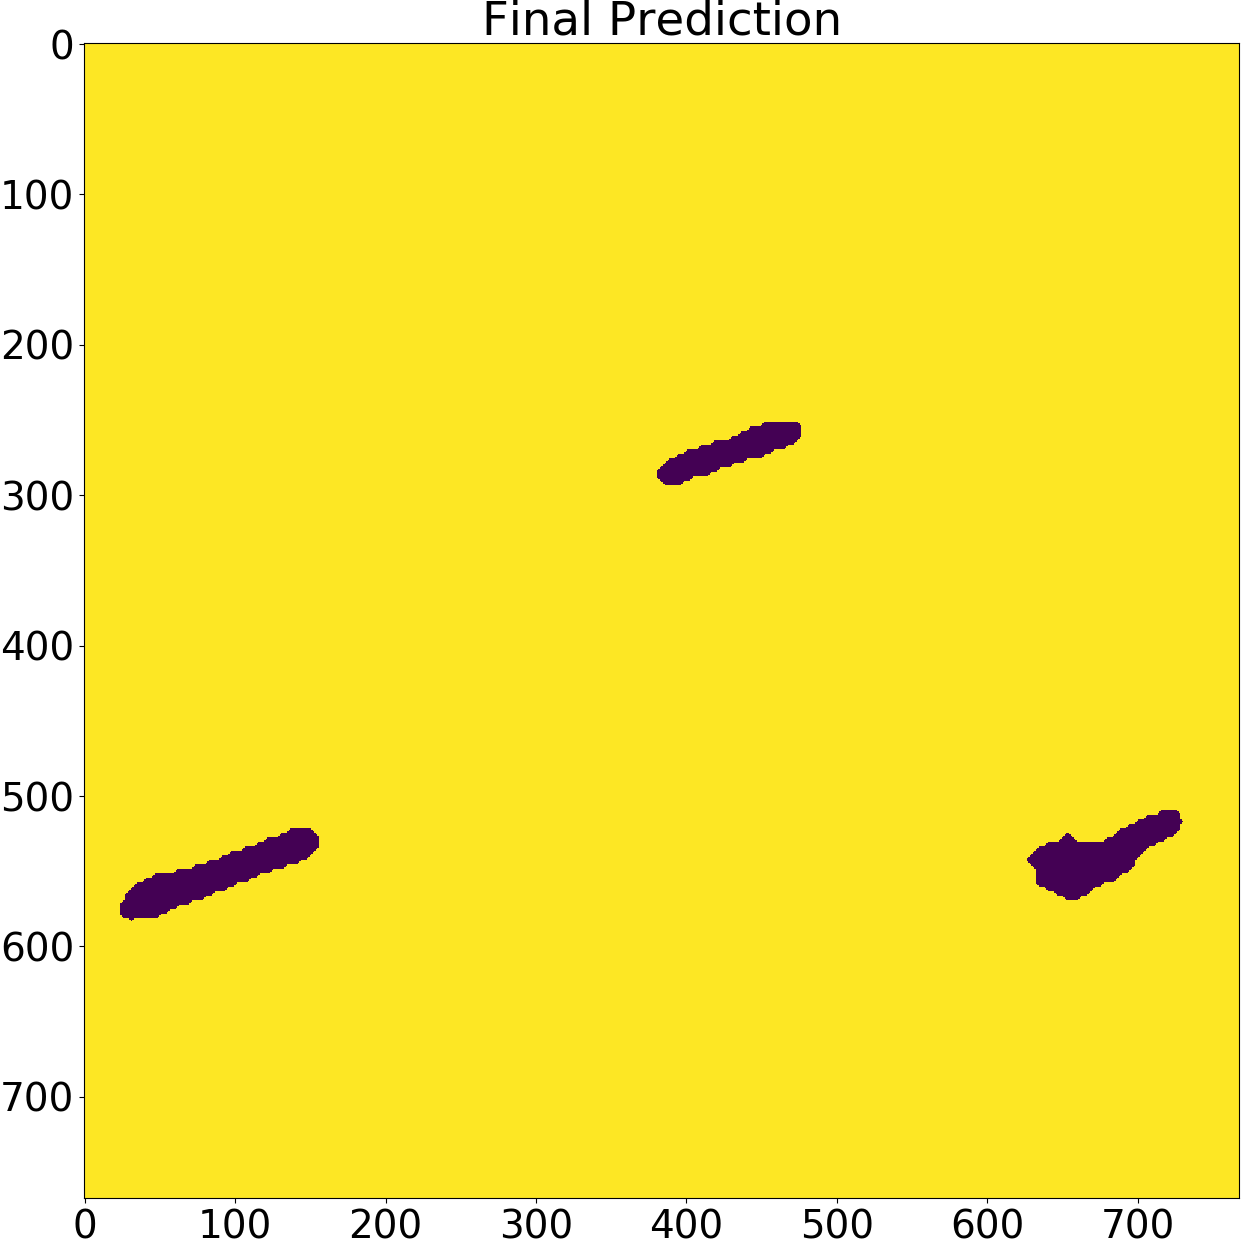
\includegraphics[width=0.45\textwidth]{Pictures/014FinalResult.png}
	\caption{Final Result}
	\label{final_result_pic_unet}
\end{figure}